\section{Experiments}

We conduct a series of experiments to comprehensively evaluate the effectiveness of LongFlow. Our evaluation focuses on three key aspects: model quality, inference speed, and memory efficiency.





\subsection{Experimental Setup}
\label{sec:setup}
\noindent\textbf{Models.}
We evaluate LongFlow on different reasoning models to demonstrate its applicability.
Our experiments are primarily conducted on \textbf{DeepSeek-R1-Distill-Llama-8B} \citep{deepseekr1} and the \textbf{Qwen3} \citep{qwen3} series, including its 0.6B, 1.7B, 4B, and 8B variants.

\noindent\textbf{Datasets.}
Our evaluation spans a wide spectrum of challenging reasoning benchmarks to ensure a comprehensive assessment of model accuracy. For competition-level mathematics, we use problems from MATH-500 \citep{hendrycks2021measuring}, AMC-23 \citep{amc}, AIME-24 \citep{aime2024} and AIME-25 \citep{aime2025}. To test advanced scientific reasoning, we employ the graduate-level expert QA from GPQA \citep{rein2024gpqa}, university-level problems from Minerva \citep{lewkowycz2022solving}, and Olympiad-level questions from OlympiadBench \citep{he2024olympiadbench}. Finally, we include the widely-used GSM8K benchmark \citep{cobbe2021training} for grade-school math word problems.

\noindent\textbf{Baselines.}
We compare LongFlow against several representative KV cache compression methods:
\begin{itemize}[itemsep=0pt,topsep=0pt,parsep=0pt]
    \item \textbf{Vanilla:} The standard attention without any KV cache management. It serves as the accuracy upper bound but represents the worst scenario for memory consumption and latency.
    
    \item \textbf{H2O}\citep{h2o}: A classic importance-based method that prioritizes tokens based on accumulated attention scores.
    
    \item \textbf{VATP}\citep{vatp}: An advanced method that integrates both attention scores and Value vector information into its importance metric.
    
    \item \textbf{R-KV}\citep{rkv}: A recent method also designed for reasoning models. It incorporates information about repetitive patterns in the generation to guide its eviction policy.
\end{itemize}

\noindent\textbf{Evaluation Metrics.}
We evaluate all methods across two primary dimensions. For system performance, we measure the inference throughput, peak GPU memory usage, and memory fragments. For model accuracy, we report the task-specific accuracy on each of the benchmarks.

\noindent\textbf{Implementation Details.}
For our main experiments, the generation output length is set to 16,000 tokens. For all compression methods, we set the KV cache budget to be either 3,200 or 2,400 tokens.
For H2O and VATP, this budget is evenly split between heavy-hitter tokens and recent tokens.
For LongFlow, if the number of tokens in the prefill stage exceeds the budget, we first use SnapKV \citep{snapkv} to compress the tokens to the budget size.
For all the baselines, we set the compression interval to achieve a balance between compression ratio and inference speed.
All the experiments are conducted on NVIDIA A100 40GB GPUs.


\subsection{Main Results on Model Accuracy}
\begin{table*}[t]
\centering
 % 使用更小的字体
\small
\renewcommand{\arraystretch}{1.2} % 稍微减小行间距
\setlength{\tabcolsep}{6pt} % 进一步减小列间距
\begin{tabular}{l|ccccccccc}
\toprule
\multirow{2}{*}{\parbox{1.8cm}{\centering\textbf{Model}}} & \multirow{2}{*}{\textbf{Method}} & \textbf{AIME24} & \textbf{AIME25} & \textbf{AMC} & \textbf{GPQA} & \textbf{GSM8K} & \textbf{MATH} & \textbf{Minerva} & \textbf{Olympiad}  \\
& & \textbf{(30)} & \textbf{(30)} & \textbf{(40)} & \textbf{(198)} & \textbf{(1318)} & \textbf{(500)} & \textbf{(272)} & \textbf{(675)} \\
\hline
\multirow{13}{*}{\parbox{1.8cm}{\centering\textbf{\shortstack{DeepSeek-R1\\-Distill1\\-Llama-8B}}}}
 & \multicolumn{9}{c}{\cellcolor{cyan!5}\textbf{Budget = 2400}} \\
& Vanilla & 30.00 & 20.00 & 77.50 & 41.41 & 77.48 & 83.40 & 20.59 & 44.30 \\
& H2O & \textbf{43.33} & \textbf{20.00} & 65.00 & \textbf{41.41} & \textbf{77.71} & 79.80 & 19.12 & 44.00 \\
& R-KV & 36.67 & 20.00 & \textbf{75.00} & 38.38 & 77.41 & \textbf{80.80} & 20.22 & \textbf{45.93} \\
& VATP & 33.33 & 13.33 & 72.50 & 33.84 & 77.48 & 79.80 & \textbf{20.59} & 43.56 \\
& Ours & 33.33 & 16.67 & 70.00 & 40.40 & 77.71 & 79.80 & 20.22 & 43.85 \\
 & \multicolumn{9}{c}{\cellcolor{cyan!5}\textbf{Budget = 3200}} \\
& Vanilla & 30.00 & 20.00 & 77.50 & 41.41 & 77.47 & 83.40 & 20.59 & 44.30 \\
& H2O & 36.67 & 23.33 & 72.50 & 38.38 & \textbf{77.69} & 81.60 & \textbf{21.32} & 46.22  \\
& R-KV & 30.00 & 23.33 & 77.50 & \textbf{42.93} & 77.62 & \textbf{82.40} & 19.49 & \textbf{46.81}  \\
& VATP & \textbf{40.00} & 16.67 & 72.50 & 42.42 & 77.39 & 81.60 & 19.12 & 46.67  \\
& Ours & 33.33 & \textbf{26.67} & \textbf{82.50} & 40.91 & 77.62 & 79.80 & 20.22 & 45.93 \\
\hline
\multirow{13}{*}{\parbox{1.8cm}{\centering\textbf{Qwen3-8B}}}
 & \multicolumn{9}{c}{\cellcolor{cyan!5}\textbf{Budget = 2400}} \\
& Vanilla & 60.00 & 46.67 & 90.00 & 34.85 & 95.68 & 92.60 & 33.46 & 58.22 \\
& H2O & 40.00 & 20.00 & 65.00 & 26.77 & 95.98 & 85.20 & 32.35 & 49.04  \\
& R-KV & 33.33 & 23.33 & \textbf{85.00} & 28.79 & 96.13 & \textbf{89.00} & \textbf{32.72} & \textbf{53.33} \\
& VATP & \textbf{40.00} & 26.67 & 77.50 & 23.23 & \textbf{96.29} & 87.60 & 31.99 & 49.33 \\
& Ours & 36.67 & \textbf{26.67} & 80.00 & \textbf{30.81} & 95.83 & 88.00 & 31.25 & 51.11 \\
 & \multicolumn{9}{c}{\cellcolor{cyan!5}\textbf{Budget = 3200}} \\
& Vanilla & 60.00 & 46.67 & 90.00 & 34.85 & 95.68 & 92.60 & 33.46 & 58.22 \\
& H2O & 46.67 & 26.67 & 80.00 & 27.78 & 96.36 & 90.40 & \textbf{35.29} & 53.78 \\
& R-KV & 50.00 & \textbf{33.33} & 82.50 & \textbf{32.32} & 96.36 & \textbf{91.60} & 33.46 & \textbf{55.56} \\
& VATP & 43.33 & 33.33 & 82.50 & 30.30 & \textbf{96.43} & 91.00 & 34.19 & 55.41 \\
& Ours & \textbf{50.00} & 26.67 & \textbf{85.00} & 30.30 & 96.36 & 89.80 & 34.19 & 55.56 \\
\bottomrule
\end{tabular}
\caption{Model Performance on different models across different datasets. Numbers in parentheses indicate dataset sizes. \textbf{Bold} indicates the best performance.}
\label{tab:model_performance}
\end{table*}

We present our main results on model accuracy in Table \ref{tab:model_performance}. The evaluation across two distinct model families and two KV cache budget settings demonstrates that LongFlow effectively preserves the reasoning capabilities of the base models, achieving performance that is highly competitive with state-of-the-art baselines and close to the uncompressed Vanilla model.

\noindent\textbf{Comparison With the Baselines.}
Across both models and budget settings, our proposed LongFlow demonstrates highly competitive performance against state-of-the-art baselines. R-KV generally achieves the highest average accuracy (with more memory for redundant token identification), establishing itself as a strong baseline focused on quality preservation. LongFlow consistently performs on par with or better than other methods like VATP and H2O. 

\noindent\textbf{Comparison with Full KV and Different Cache Budgets.}
A key finding is that all compression methods, including LongFlow, successfully preserve the vast majority of the original model's capabilities while operating on a significantly reduced KV cache (e.g., a 3.2k budget representing an 80\% compression ratio for a 16k generation).
As shown in Table \ref{tab:model_performance}, the average performance degradation compared to the uncompressed Vanilla baseline is negligible to minor—as low as 0.08\% for DeepSeek-R1-Distill-Llama-8B and approximately 1.3\% for Qwen3-8B.
When the KV cache budget is tightened from 3.2k to 2.4k, a graceful degradation is observed across all methods. LongFlow performs better under this pressure, showing less degradation than both H2O and VATP.

\subsection{Performance on Different Model Sizes}
To assess the performance of LongFlow across different model sizes, we conduct a comparative analysis using the Qwen3 model family, including the 0.6B, 1.7B, 4B, and 8B variants.
For this specific analysis, the AIME-24 and AIME-25 datasets were excluded due to their small sample sizes and for brevity.
The results in Figure \ref{fig:all_images} (in Appendix \ref{sec:additional figures}) show that LongFlow maintains a highly competitive performance, achieving results that are comparable or superior to the baselines across all tested model sizes and benchmarks, which demonstrates the effectiveness and robustness of our method.



\begin{figure*}[t]
\centering
\begin{subfigure}[b]{0.32\textwidth}
    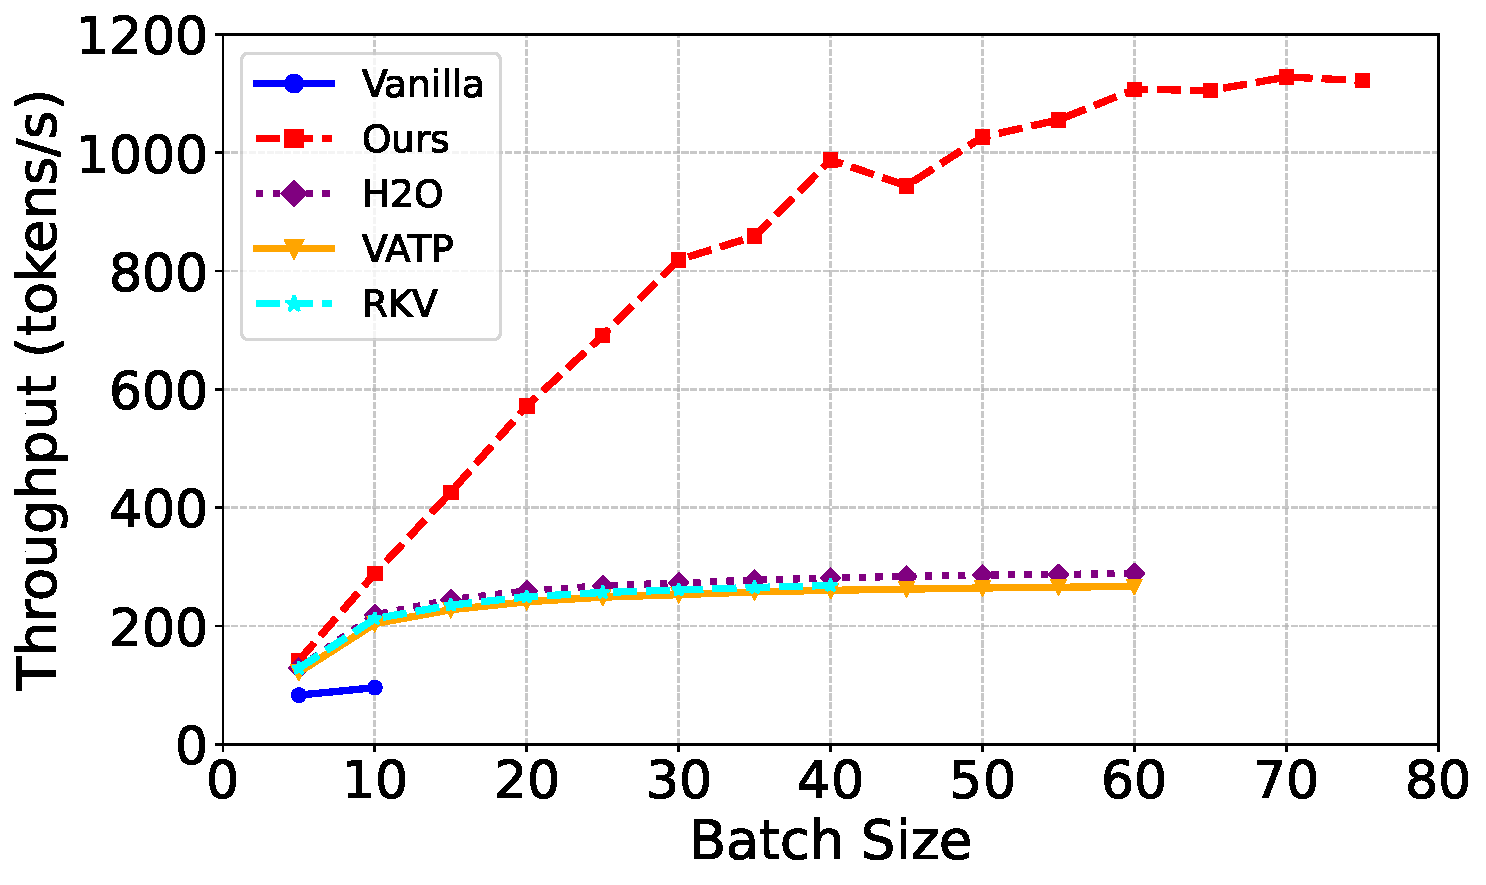
\includegraphics[width=\textwidth]{figure/throughput_comparison.pdf}
    \caption{Throughput}
\end{subfigure}
\begin{subfigure}[b]{0.32\textwidth}
    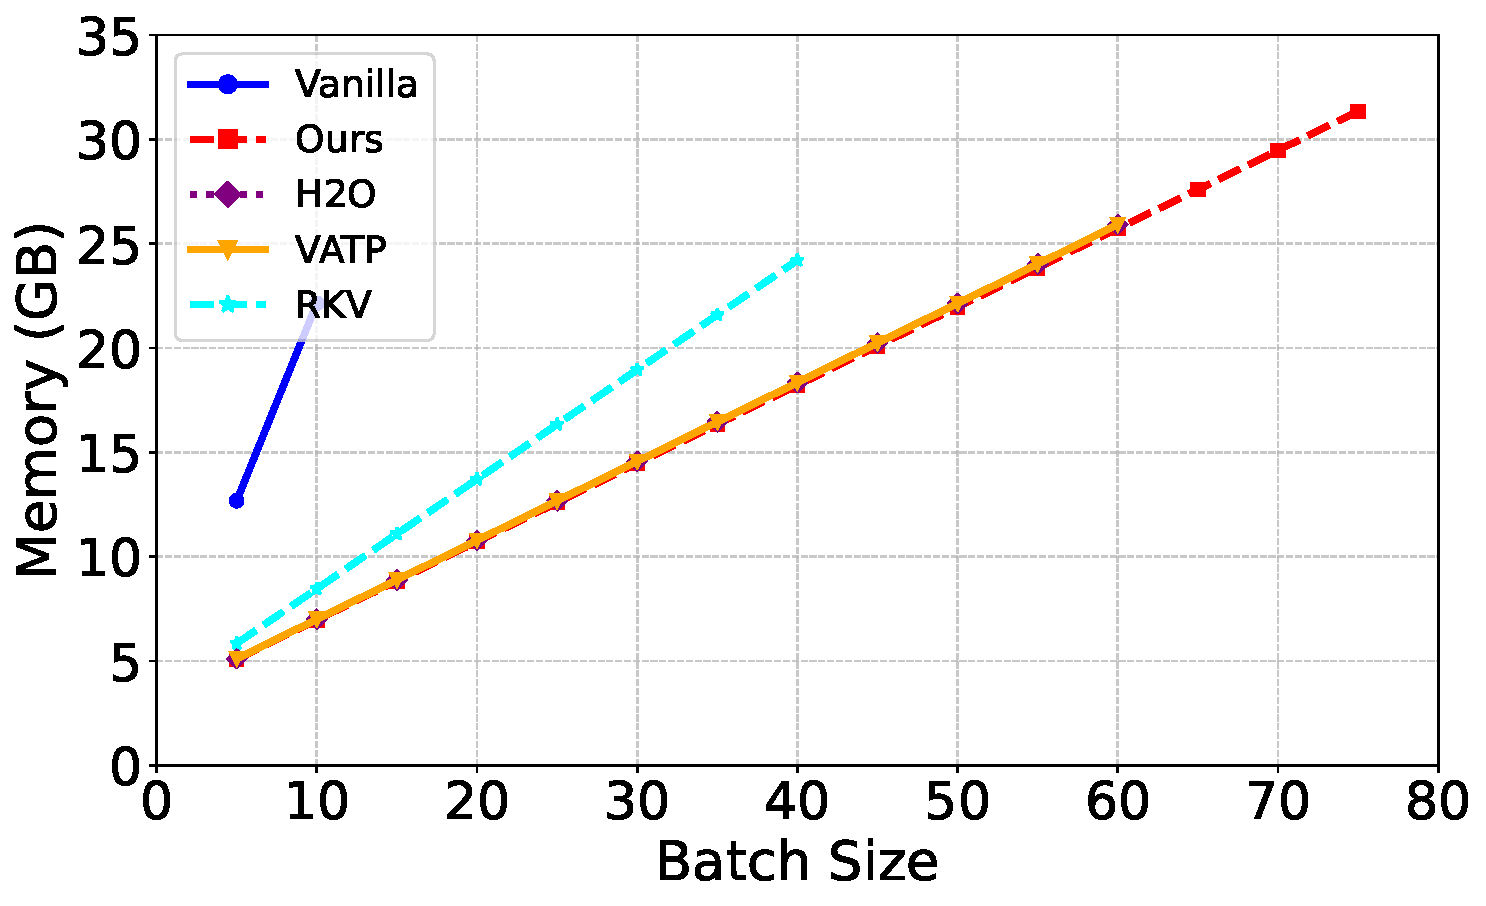
\includegraphics[width=\textwidth]{figure/memory_comparison.pdf}
    \caption{Memory usage}
\end{subfigure}
\begin{subfigure}[b]{0.32\textwidth}
    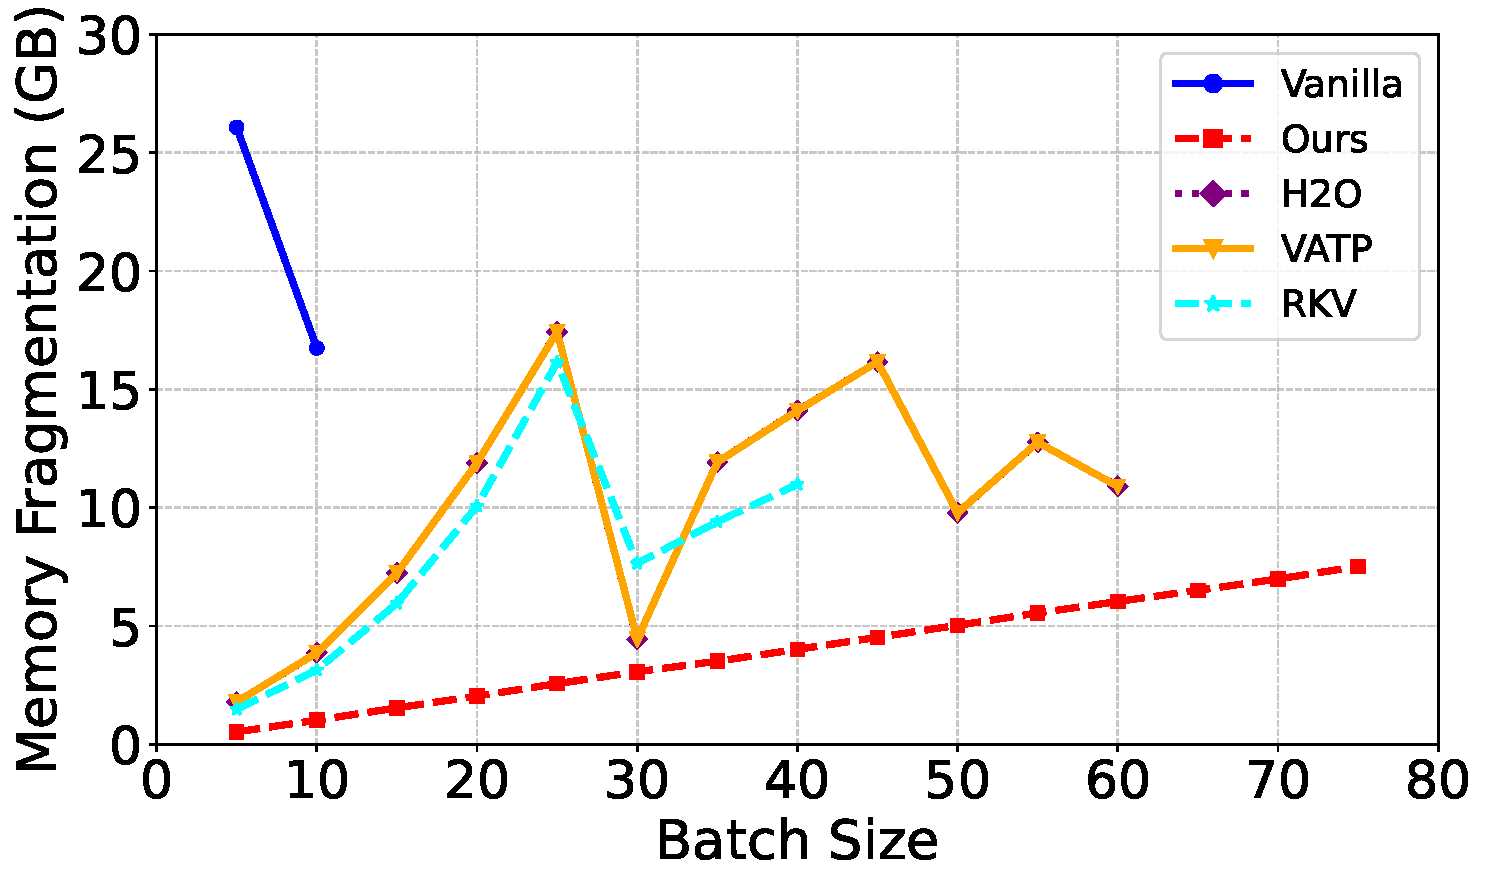
\includegraphics[width=\textwidth]{figure/gpu_memory_diff_comparison.pdf}
    \caption{Memory fragment}
\end{subfigure}
\caption{Performance comparison of LongFlow against baselines. The compression is conducted every step for LongFlow and every 128 steps for other methods. LongFlow achieves higher throughput and supports a larger maximum batch size due to superior memory management.}
\vspace{-10pt}
\label{fig:memory_and_speed}
\end{figure*}

\subsection{Throughput and Memory Analysis}
Finally, we evaluate the system-level performance of LongFlow in terms of throughput and memory efficiency. For this analysis, we use the Qwen3-1.7B on a single NVIDIA A100 40GB GPU. We configure a scenario with an input length of 512 and an output length of 16,000. We set the KV cache budget to 3,200 for all compression methods. To measure the maximum performance, we progressively increase the batch size for each method until an Out-of-Memory (OOM) error occurs. We report the throughput, peak memory footprint, and memory fragments in Figure \ref{fig:memory_and_speed}.


The results clearly demonstrate LongFlow's substantial advantages in both throughput and memory management. In terms of throughput, LongFlow outperforms FullKV by a remarkable 11.8 times and is approximately 4.0 times faster than other methods.
Although LongFlow performs KV cache compression at every decoding step, its algorithmic efficiency and fused kernel implementation substantially reduce per-step overhead, enabling remarkably higher throughput than competing methods.
Regarding peak memory usage, LongFlow's footprint is comparable to other methods under the same budget, while R-KV consumes slightly more due to its more complex importance estimation logic.
Notably, LongFlow's advantage in memory management lies in its superior handling of fragmentation. Its static memory scheme and consistent per-step eviction policy result in a memory layout that is both less fragmented and highly predictable.
This less fragmented memory layout allows LongFlow to support a larger maximum batch size than competing methods.
The predictability makes LongFlow more stable and reliable in real-world deployment by eliminating runtime memory-related uncertainties,.


